\documentclass[a4paper, 10pt,twoside]{report}
\usepackage[utf8x]{inputenc}

% english language
\usepackage[UKenglish]{babel}

% ps tricks
\usepackage[usenames,dvipsnames]{pstricks}

% about title
\usepackage{titlesec}

% margins
\topmargin 0cm
\headsep 1cm
\headheight 0.6cm
\textwidth 16.6cm
\textheight 21.8cm
\evensidemargin -0.5cm
\oddsidemargin -0.5cm

% mathematics
\usepackage{amsmath}
\usepackage{amsfonts}


% definition
\usepackage{amsthm}
\theoremstyle{plain}
\newtheorem{thm}{Theorem}[section]
\newtheorem{cor}[thm]{Proof.}

\theoremstyle{definition}
\newtheorem{defn}{Definition}[section]

\theoremstyle{remark}
\newtheorem{rmk}{Remark}

% test format
\usepackage{verbatim}
\usepackage{color}
\usepackage{eurosym}

% symbols
\usepackage{textcomp, latexsym, amssymb, gensymb, placeins}
\usepackage[mathscr]{euscript}
\usepackage{amsmath}

% figures
\usepackage{epsfig}
\usepackage{graphics, epsfig, color, colortbl, supertabular}
\usepackage{subfigure}
\usepackage{epstopdf}

% tables
\usepackage{multirow, ctable, rotating, lscape}
\usepackage{array}
\usepackage{booktabs}
\usepackage{supertabular}
\usepackage{tabularx}
\usepackage{graphicx}

% other packages
\usepackage{hyperref}
\def\thesection{\arabic{section}}
\def\theequation{\arabic{equation}}

\addtocounter{section}{1}
\setcounter{secnumdepth}{3}
\setcounter{tocdepth}{3}
\setcounter{section}{0}

\usepackage{float}
\usepackage{stmaryrd}


% tikz
\usepackage{tikz}
\usetikzlibrary{mindmap,trees}
\usetikzlibrary{arrows,decorations.pathmorphing,backgrounds,fit,positioning,%
  shapes.symbols,chains}
\usetikzlibrary{calc,trees,positioning,arrows,chains,shapes.geometric,%
  decorations.pathreplacing,decorations.pathmorphing,shapes,%
  matrix,shapes.symbols}


% acronyms
\usepackage{acronym}


% URL
\usepackage{url}

\usepackage{fancyhdr}
\usepackage{etex}
\usepackage{epstopdf}

% X Quartapelle
% \renewcommand{\theequation}{\thechapter.\arabic{equation}}
% \newcommand{\clearemptydoublepage}{\newpage{\pagestyle{empty}
% \cleardoublepage}}
\renewcommand{\headrulewidth}{0.3pt}
\renewcommand{\footrulewidth}{0.3pt}
\newcommand{\virgolette}[1]{``#1''}

% Mathematical Operator
\newcommand{\WE}{\mathcal{W}}
\newcommand{\W}{$\mathcal{W}$}
\newcommand{\LE}{\mathcal{L}}
\newcommand{\Lne}{$\mathcal{L}$}
\newcommand{\delOp}{\widehat{\boldsymbol{\nabla}}}
\newcommand{\diver}[1]{\text{Div}\big(#1\big)}
\newcommand{\invariants}{$\big(I_{\C},II_{\C},III_{\C}\big)$}

% Eucledian spaces
\newcommand{\Real}{$\mathbb{R}^3$}
\newcommand{\RN}{\mathbb{R}^{N_h}}

% Lagrangian and Eulerian displacements
\newcommand{\displL}{\widehat{\underline{\eta}}}
\newcommand{\displE}{\underline{\eta}}

% Discrete displacement, velocity and acceleration
% The fist command is to reuse the same already existing formula
\newcommand{\Spost}{\widehat{\underline{\Lambda}}}
\newcommand{\GradSpost}{\delOp\delta\Spost}
\newcommand{\vectL}{\widehat{\underline{\Lambda}}}
\newcommand{\velVect}{\widehat{\underline{W}}}
\newcommand{\acc}{\widehat{\underline{A}}}

% Stiffness Vectors, discretized system
\newcommand{\StiffVect}{\underline{K}(\vectL)}
\newcommand{\StiffDiscr}[1]{\underline{K}(\vectL^{#1})}

% Lagrangian velocity
\newcommand{\velL}{\widehat{\underline{v}}}
\newcommand{\velE}{\underline{v}} %Test function (velocity)
\newcommand{\velwE}{\widehat{\underline{w}}}

% Programming names
\newcommand{\SSol}{\textit{Structural Solver}}
\newcommand{\SSolNC}{Structural Solver}
\newcommand{\LV}{\texttt{LifeV}}
\newcommand{\tPC}[1]{\texttt{#1}}
\newcommand{\AES}{AssemblyElementalStructure}
\newcommand{\tSS}{\textit{test\_structuralsolver}}

% Reference and Current Configuration
\newcommand{\RefCon}{$\mathcal{B}_0$}
\newcommand{\CurCon}{$\mathcal{B}(t)$}
\newcommand{\RefConE}{\mathcal{B}_0}
\newcommand{\CurConE}{\mathcal{B}(t)}

% Position in the reference and current configuration
\newcommand{\posE}{\underline{X}}
\newcommand{\nposE}{\underline{x}}
\newcommand{\pos}{$\underline{X}$}
\newcommand{\npos}{$\underline{x}$}

% Tensors and matrices
\newcommand{\F}{\textbf{F}}
\newcommand{\cofF}{\text{Cof}\textbf{F}}
\newcommand{\T}{\textbf{T}}
\newcommand{\D}{\textbf{D}}
\newcommand{\C}{\textbf{C}}
\newcommand{\Cbar}{\bar{\textbf{C}}}
\newcommand{\I}{\textbf{I}}
\newcommand{\mass}{\textbf{M}}
\newcommand{\Piola}{\textbf{P}}
\newcommand{\Et}{\textbf{E}}

% Expression for the Exponential-Material
\newcommand{\term}{e^{\gamma\left(I_{\C}-3\right)}}

\newtheorem{weak}{Weak-formulation}[chapter]
\newtheorem{problem}{Problem}[chapter]

% Title Page
\title{Structural Solver framework in \textit{LifeV}:
Description and Usage}
\author{Paolo Tricerri, Gianmarco Mengaldo}


\begin{document}

\maketitle


\section*{Summary} The aim of the present document is to describe the
\SSol framework in the open source finite element library LifeV. This
framework has been developed to have a unique solver for structural
dynamics problems (described by the equation of motion) letting the
users plug different constitutive laws into the conservation
equation of linear momentum in a flexible way.\\ In this report, we
aim at:
\begin{itemize}
\item presenting the architecture of the StructuralSolver;
\item giving a detailed description of the constitutive laws
  implemented;
\item showing the usage of \textit{test\_structuralsolver} that has
  been developed and, to conclude, presenting the validation of the
  implemented laws, with respect to analytical and semianalytical
  solutions;
\end{itemize} This document is divided in different sections. The
first one briefly introduces the continuum mechanics theory behind the
formulation of the conservation equation of linear momentum. After
that, the mathematical formulation of the constitutive laws available
in the library is presented. The second section deals with the
discretization of the continuous differential problem and its
formulation in the finite element method. Moreover, the linearization
of the nonlinear algebraic system at each time step is shown. The
third part describes the main features of the \SSol framework and the
implementation of the constitutive laws defined in the first
section. The last section describes the
\textit{test\_structuralsolver} for a user who wants to solve
structural dynamics problems. Starting from the case solved in the
test, the section deals with the validation of the different material
laws, with respect to an analytical and semianalytical solution for a
traction test on a cube.\\

\section*{Acknowledgements} The authors would like to thank
Dr. Mariarita Deluca for her help during the development and debug of
the code and for implementing a first version of the structural models
in the serial version of the library.

\tableofcontents
\newpage


\section{Continuum mechanics and Constitutive laws} This section deals
with the derivation and formulation of the conservation equation of
linear momentum and the description of the constitutive laws available
in \LV.

\subsection{Continuum mechanics}
\label{sct-Continuum} In order to describe the motion and deformations
of a body, we embed it in a three-dimensional Eucledian space. Let
\RefCon $\subseteq$ \Real be the \textit{reference configuration} of
the body. This enables us to uniquely identify any arbitrary point
$P(\posE)$, called \textit{material point}, in \RefCon by its position
at the initial time $t_0=0$. When the body moves, at each time $t>0$,
it will occupy a new configuration \CurCon, which will be called the
\textit{current configuration}. In the study of the kinematics of a
body, it is commonly assumed that the motion of an arbitrary material
point, starting from \pos, can be described through a relationship of
the form:
\begin{equation} \nposE=\chi(\posE,t)\qquad t\geq0,
  \label{eq::deformation}
\end{equation} where \npos is the new position of the point \pos,
$\chi$ is a continuously differentiable function in all variables (at
least up to the second derivatives). Moreover, we assume that at each
time $t>0$, the following property on $\chi$ holds: for any \pos and
corresponding point \npos, there are open balls $B_{\posE}$ (centered
in \pos) and $B_{\nposE}$ (centered in \npos), both contained in
\RefCon and \CurCon, such that points in $B_{\posE}$ are in one-to-one
correspondance with points of $B_{\nposE}$.\\ Thanks to the map
\eqref{eq::deformation} we can define the displacement of a point
$P(\posE,t_0=0)$ at time $t>0$ as
\begin{equation} \displL=\nposE(\posE,t)-\posE
  \label{eq::displacementL}
\end{equation} It is worth noticing that the displacement field has
been defined in the Lagrangian framework. Its Eulerian description is
given by:
\begin{equation} \displE=\nposE-\chi^{-1}(\nposE,t).
  \label{eq::displacementE}
\end{equation} According to these two representations, it is possible
to define other kinematics quantities (e.g. velocity and acceleration
fields) in each of the two coordinate systems.\\ The local deformation
of a material point is characterized by a second order tensor, usually
indicated by \F and called \textit{deformation gradient}, which is
defined as:
\begin{equation} \F = \delOp\nposE,
  \label{eq:tensorF}
\end{equation} where the symbol $\delOp$ indicates that the
derivatives are computed with respect to the coordinates in the
reference configuration. In addition, the tensor \F allowsfor defining
other classical tensorial quantities, like the right Cauchy-Green and
Green-Lagrange tensors, to quantify the stretches and strains during
the deformation.\\

\subsubsection{Conservation equation of linear momentum}
\label{sct-Conservation} The postulate of balance of linear momentum
states that the rate of change of linear momentum of a fixed mass of
the body is equal to the sum of the forces acting on the body. These
forces can derive from as body forces or as forces due to stress
vectors acting on the surface of the body,
\begin{equation} \frac{d}{dt}\int_{\CurConE}\rho\velE dv =
  \int_{\CurConE}\rho\underline{b}
  dv+\int_{\partial\CurConE}\underline{t}da
  \label{eq::BLM-IntegralFormEulerian}
\end{equation} where $\rho$ is the density of the material in the
current configuration (and it is related to its counterpart in \RefCon
thanks to $\rho=J\rho_0$) and $\velE$ is the Eulerian velocity. The
vector $\underline{b}$ is the body force per unit of mass,
$\underline{t}=\underline{t}(\nposE,t, \underline{n})$ is the surface
force acting on the body in the current configuration per unit area of
$\partial\CurConE$ and $\underline{n}$ is the outward unit normal to
the surface $\partial\CurConE$ at \npos at time $t$. The first and the
second integrals on the right hand side represent the contributions
due to body forces and to surface forces, respectively.\\ The surface
tension $\underline{t}$, thanks to the Cauchy lemma and the relation
between the stress tensor and the stress vector, can be written as:
\begin{equation} \underline{t}=\underline{t}(\nposE,t,
  \underline{n})=\T(\nposE,t)\underline{n}.
  \label{eq::tension}
\end{equation} Substituing \eqref{eq::tension} in
\eqref{eq::BLM-IntegralFormEulerian} and using the divergence theorem,
equation \eqref{eq::BLM-IntegralFormEulerian} becomes:
\begin{equation} \frac{d}{dt}\int_{\CurConE}\rho\velE dv =
  \int_{\CurConE}\big(\rho\underline{b} +\text{div}\T \big)dv.
  \label{eq::BLM-Eulerian}
\end{equation} Equation \eqref{eq::BLM-Eulerian} is the Eulerian
integral form of the conservation equation of linear momentum. In
order to write it in its Lagrangian form we need to compute the
integrals on the reference configuration \RefCon. Using the identities
$dv=JdV$, $\rho=J\rho_0$, $da=J\F^{-T}dA$, where $J=\text{det}\F$, and
remembering the definition of the First Piola-Kirchhoff tensor
($\Piola=J\T\F^{-T}$), the Lagrangian form of
\eqref{eq::BLM-IntegralFormEulerian} is:
\begin{equation} \frac{d}{dt}\int_{\RefConE}\rho_0\velL dV =
  \int_{\RefConE}\big(\rho_0\underline{b}+\text{Div}\Piola \big)dV,
\end{equation} where $\velL$ is the Lagrangian velocity and
$\text{Div}(\cdot)$ is the divergence operator in the material
coordinates. Assuming a constant density both in space and time, the
local Lagrangian form of the conservation equation of linear momentum
is:
\begin{equation} \rho_0\frac{\partial^2\displL}{\partial
    t^2}=\rho_0\underline{b}+\text{Div}(\Piola) \qquad \forall \posE
  \subseteq \RefConE, \quad t>0.
  \label{eq::ConLinMom-Diff}
\end{equation} When initial and boundary conditions are added to
Eq. \eqref{eq::ConLinMom-Diff} the mathematical problem associated to
\eqref{eq::ConLinMom-Diff} of structural mechanics is
defined. Subsequentely, this problem is characterized by specifying a
particular constitutive law for the Cauchy stress tensor.

\subsection{Constitutive laws}
\label{sct-Constitutive} Equation \eqref{eq::ConLinMom-Diff} must be
closed by an adequate constitutive law in order to have a solveable
mathematical problem. The closure equation relates the Cauchy stress
tensor \T to the deformation gradient \F. The most general form of
this kind of relation is:
\begin{equation} \T(\nposE)=\mathcal{G}\big(F(\nposE,t),\nposE\big).
  \label{eq::GeneralCL}
\end{equation} In the following we will consider Cauchy elastic
materials (i.e. materials in which the current stresses in \CurCon are
determined only by the current state of deformation) and homogeneous
materials (i.e. the material behaviour is independent of the material
point). Under these hypothesis, relation \eqref{eq::GeneralCL} reduces
to the form
\begin{equation} \T(\nposE)=\mathcal{G}\big(F(\nposE,t)\big),
  \label{eq::OurRelation}
\end{equation} where $\mathcal{G}$ is called the response function.\\
The structural models which have been implemented in the \SSol
framework are for isotropic hyperelastic materials. A material is said
to be hyperelastic when it does not dissipate energy during cyclic
homogeneous deformations,
\begin{equation} \text{W}_{\text{cycle}} =
  \int_{0}^{\text{T}}\int_{\RefConE}\,\mathbf{P}:\dot{\mathbf{F}}\,d\RefConE\text{dt}
  = 0,
  \label{eq::energyDiss}
\end{equation} along any deformation characterized by
$\posE(t=T)=\posE(t=0)$ at any point of \RefCon. For hyperelastic
materials, the stress power can be represented in the following way:
\begin{equation} \rho\frac{D\WE(\posE,t)}{Dt}=\T:\D
  \label{eq::HyperSP}
\end{equation} where \D is the velocity gradient tensor and \W is the
\textit{strain energy density function}. This function characterizes
one particular material from another. From the mathematical point of
view, the strain energy function of an isotropic hyperelastic material
is a function of the right Cauchy-Green tensor ($\C=\F^{T}\F$) and, in
particular, without loss of generality, \W can be written in terms of
the invariants of \C,
\begin{equation} \WE=\WE\big(I_{\C},II_{\C},III_{\C}\big).
  \label{eq::WandInvariants}
\end{equation} All the tensors (e.g. \F,\T,\Piola) which describe the
mechanical response of this kind of materials can be computed by
derivation of \W with respect to $I_{\C},II_{\C},III_{\C}$ and \C.This
theory will not be discussed in depth in this report, but a more
detailed explanation can be found in \cite{GM,Deluca} and references
therein. We would, however, like to remind that in order to guarantee
the well posedness of the structural mechanic problem
\eqref{eq::ConLinMom-Diff} the strain energy function \W of the
material has to satisfy the condition of policonvexity.\\ In the
following we will characterize the strain energy function for all the
four stress-strain relations which are available in \LV and we will
give the corresponding expression of the first Piola-Kirchhoff
tensor. In particuar, the first two models that we analyze describe
isotropic hyperelastic compressible material and the second two
isotropic hyperelastic nearly-incompressible materials. Since the
applications we are interested in concern models of incompressible
materials, we will enforce the incompressibility constraint in our
simulations:
\begin{itemize}
\item by using high Poisson ratios for the first two
  models\footnote{The choice of high Poisson ratios may be critical in
    terms of a well-known problem: locking.}
\item by recovering the common multiplicative decomposition of the
  deformation gradient \F into an isochoric and volumetric part for the
  second two (see \cite{BonetWood}).
\end{itemize} In the following subsections, the computations for the
definition of the first Piola-Kirchhoff tensor will not be detailed
here, but can be found in \cite{Deluca} and references therein.

\subsubsection{St. Venant-Kirchhoff and Linear Elastic models} Both of
these models take origin from the same strain energy function. The
characteristic function \W for these two constitutive laws is:
\begin{equation} \WE\big(\Et\big)=\frac{\lambda}{2}(\text{tr}\Et)^2 +
  \mu\Et:\Et
  \label{eq::W-SVKLE}
\end{equation} where \Et is the Green-Lagrange tensor and it is
defined as $\Et=\frac{1}{2}\big(\C-\textbf{I}\big)$, and $\lambda$ and
$\mu$ are the first Lam\'e constant and the shear modulus
respectively. These two materials parameters are functions of the
Young modulus E and Poisson ratio $\nu$ as follows:
\begin{equation} \lambda=\frac{\nu E}{\big(1+\nu \big)\big(1-2\nu
    \big)}\qquad\qquad \mu=\frac{E}{2\big(1+\nu\big)}.
  \label{eq::LameConst}
\end{equation} Since the material is hyperelastic and isotropic, as we
said earlier, \W can be written in terms of the invariants of \C,
leading to the relation:
\begin{equation}
  \WE=\left(\frac{\lambda}{8}+\frac{\mu}{4}\right)I_{\C}^2 -
  \left(\frac{3\lambda}{4}+\frac{\mu}{2}\right)I_{\C} -
  \frac{\mu}{2}II_{\C}+\frac{9\lambda}{8}+\frac{3\mu}{4}
  \label{eq::WSVK-Inv}
\end{equation} For the St. Venant-Kirchhoff material the first
Piola-Kirchhoff tensor is:
\begin{equation} \Piola = \frac{\lambda}{2}\big(I_{\C}-3\big)\F +
  \mu\F +\mu\F\C
  \label{eq::SVK-P}
\end{equation} It is convenient to introduce the displacement field,
$\displL$, in the expression \eqref{eq::SVK-P} which transforms into:
\begin{equation}
  \begin{array}{llll} \Piola(\displL) = & \displaystyle
    \lambda(\diver{\displL})\I + \mu\big(\delOp\displL +
    \delOp\displL^T\big)
    +\frac{\lambda}{2}\big(\delOp\displL:\delOp\displL\big)+ \\ \\ &
    \displaystyle + \lambda\big(\diver{\displL}\big)\delOp\displL +
    \frac{\lambda}{2}\big(\delOp\displL:\delOp\displL\big)\delOp\displL +
    \mu\big(\delOp\displL^T \delOp\displL\big)+\\ \\ & \displaystyle +
    \mu\delOp\displL\big(\delOp\displL\delOp\displL^T\big) +
    \mu\delOp\displL\delOp\displL^T\delOp\displL.
  \end{array}
  \label{eq::SVK-P-displ}
\end{equation} which is the expression we have to insert in
\eqref{eq::ConLinMom-Diff} when we want to solve the structural
dynamic problem using the St. Venant-Kirchhoff constitutive law.\\ The
linear elastic model can be deduced from \eqref{eq::SVK-P-displ}
considering only the linear terms. In this case, the tensor \Piola is:
\begin{equation} \Piola(\displL) = \lambda(\diver{\displL})\I +
  \mu\big(\delOp\displL + \delOp\displL^T\big).
  \label{eq::LE-P}
\end{equation} It is worth to note that the St. Venant-Kirchhoff
strain energy function \eqref{eq::W-SVKLE} does not satisfy the
policonvexity condition for all the state of deformations. For this
reason, it is not recommended when large compressive strains
occur. More details can be found in \cite{Hozapfel}.

\subsubsection{Neohookean model} The expression of \W in terms of the
invariants for the Neo-Hookean material is:
\begin{equation}
  \WE=\frac{\mu}{2}\big(I_{\Cbar}-3\big)+\frac{\kappa}{4}\left[\big(J-1)^2
    + (\text{ln}J)^2\right],
  \label{eq::strainNH}
\end{equation} where $I_{\Cbar}$ is the trace of the isochoric part of
\C, $\mu$ is the shear modulus, $\kappa$ is the bulk modulus, and $J$
is the determinant of \F. In this case, the tensor \Piola reads:
\begin{equation}
  \begin{array}{lll} \Piola = & \displaystyle \mu
    J^{-\frac{2}{3}}\left(\F-\frac{1}{3}I_{\Cbar}\F^{-T}\right) +\\ \\ &
    \displaystyle +
    J\frac{\kappa}{2}\left(J-1+\frac{1}{J}\text{ln}J\right)\F^{-T}.
  \end {array}
  \label{eq::NH-P}
\end{equation} The first term in Eq. \eqref{eq::NH-P} representes the
isochoric part of \Piola, while the second is the volumetric
part. This is due to the multiplicative decomposition of
\F. Introducing the displacement field, the expression above becomes:
\begin{equation}
  \begin{array}{lll} \Piola(\displL) = & \displaystyle \mu
    J^{-\frac{2}{3}}\left(\delOp\displL -
      \frac{1}{3}\big(\delOp\displL:\delOp\displL+2\diver{\displL}+3\big)\delOp\displL^{-T}\right)+\\
    \\ & \displaystyle +
    J\frac{\kappa}{2}\left(J-1+\frac{1}{J}\text{ln}J\right)\delOp\displL^{-T},
  \end{array}
  \label{eq::NH-P-displ}
\end{equation} where we have used the identity:
\begin{equation} I_{\Cbar}=\text{tr}\Cbar=\delOp\displL:\delOp\displL
  + 2\diver{\displL}+3.
  \label{eq::Id-trC-displ}
\end{equation} The Neohookean material satisfies the policonvexity
condition for all the states of deformations. Hence, the mathematical
problems generated by Eq. \eqref{eq::ConLinMom-Diff} is well posed.

\subsubsection{Exponential model} In this case, the relation between
\W and the invariants of the isochoric part of \C is the following:
\begin{equation} \WE= \displaystyle
  \frac{\alpha}{2\gamma}\left(e^{\gamma(\I_{\Cbar}-3)}-1\right) +
  \frac{\kappa}{4}\left[\big(J-1)^2 + (\text{ln}J)^2\right],
  \label{eq::strainExp}
\end{equation} where $\alpha$ and $\gamma$ are material parameters and
$\kappa$ is, as before, the bulk modulus. After some computations, the
expression of the first Piola-Kirchhoff tensor is:
\begin{equation}
  \begin{array}{lll} \Piola = & \displaystyle \alpha
    J^{-\frac{2}{3}}\left(\F-\frac{1}{3}I_{\Cbar}\F^{-T}\right)e^{\gamma\big(I_{\Cbar}-3\big)}
    +\\ \\ & \displaystyle +
    J\frac{\kappa}{2}\left(J-1+\frac{1}{J}\text{ln}J\right)\F^{-T}.
  \end {array}
  \label{eq::EXP-P}
\end{equation} Introducing in \eqref{eq::EXP-P} the displacement
field, the expression of \Piola as a function of $\displL$ is
obtained. The first term in Eq. \eqref{eq::EXP-P} is the isochoric
contribution and the second one the volumetric. As for the Neohookean
law, the policonvexity condition is satisfied for all the state of
deformations leading to the well posedness of the mathematical problem
\eqref{eq::ConLinMom-Diff}.

\section{Finite Element Formulation}
\label{sct-FEF} \LV is a finite element library. We need to formulate
the mathematical problem related to Eq. \eqref{eq::ConLinMom-Diff} in
the framework of the finite element method. In this section we
introduce the continuous weak formulation and its approximation by the
Galerkin method. After this, we will describe the nonlinear problem
that has to be solved (using a Newton method) at each time step of the
simulation. Its linearization is presented, and the Jacobian of the
nonlinear operator is shown for each of the four constitutive laws.

\subsection{Weak formulation of the structural mechanic problem}
\label{sct-ContinuousWF} In order to derive the weak formulation of
the problem related to Eq. \eqref{eq::ConLinMom-Diff} we need first to
define it. Fig. \ref{fig::Domain} represents the domain of the
problem. The domain defined by the dashed line is the reference
configuration \RefCon and the one delimited by the solid line is the
current configuration \CurCon. The portion of the boundary $\Gamma _D$
is where Dirichlet boundary conditions are applied and $\Gamma_{N_i}$
($i=1,2$) are the portions of $\partial \RefConE$ where Neumann
boundary conditions are applied. It is worth to note that the
mathematical structural dynamic problem is defined on \RefCon since
\eqref{eq::ConLinMom-Diff} has been written in the Lagrangian
framework.

\begin{figure}[h!]  \centering
  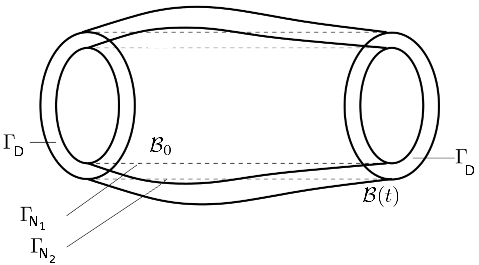
\includegraphics{images/Structure.pdf}
  \caption{Domain of the structural problem \eqref{eq::MathProb}}
  \label{fig::Domain}
\end{figure}

The differential problem is:
\begin{equation} \left\{
\begin{array}{lllllll} \displaystyle
\rho_0\frac{\partial^2\displL}{\partial
t^2}=\rho_0\underline{b}+\text{Div}(\Piola) & \text{on} \quad \RefConE
\vee t>0,\\ \\ \displL(0)=\displL_0 & \text{on} \quad \RefConE \vee
t=0,\\ \velL(0)=\velL_0 & \text{on} \quad \RefConE \vee t=0,\\
\displL(t)=\underline{0} & \text{on} \quad \Gamma_D, \quad t>0,\\
\Piola\underline{n}_1=\underline{0} & \text{on} \quad \Gamma_{N_1},
\quad t>0,\\ \Piola\underline{n}_2=\underline{t}_0 & \text{on} \quad
\Gamma_{N_2}, \quad t>0.\\
\end{array}\right.
\label{eq::MathProb}
\end{equation} If we consider the equation of motion in
\eqref{eq::MathProb}, multiply it by an arbitrary velocity field
$\velwE$ and integrate the equation on \RefCon, we get:
\begin{equation} \displaystyle \int_{\RefConE}\rho_0\frac{\partial^2
\displL}{\partial t^2}\cdot\velwE\quad d\RefConE =
\int_{\RefConE}\diver{(\Piola(\displL)}\cdot\velwE\quad d\RefConE +
\int_{\RefConE}\rho_0\underline{b}\cdot\velwE\quad d\RefConE
  \label{eq::firstIntegral}
\end{equation} Applying the divergence theorem to the first integral
at the right hand side and taking into account the boundary conditions
in \eqref{eq::MathProb} the integral relation
\eqref{eq::firstIntegral} becomes:
\begin{equation}
  \begin{array}{lll} \displaystyle
\int_{\RefConE}\rho_0\frac{\partial^2 \displL}{\partial
t^2}\cdot\velwE\quad d\RefConE & = \displaystyle -
\int_{\RefConE}\Piola(\displL):\delOp\velwE\quad d\RefConE + \\ \\ &
\displaystyle + \int_{\partial
\RefConE}\underline{t}_0\cdot\velwE\quad d\partial\RefConE +
\int_{\RefConE}\rho_0 \underline{b}\cdot\velwE\quad d\RefConE
    \end{array}
  \label{eq::secondIntegral}
\end{equation} which can be written in this form,
\begin{equation}
  \begin{array}{lll} & \displaystyle
\int_{\RefConE}\rho_0\frac{\partial^2 \displL}{\partial
t^2}\cdot\velwE\quad d\RefConE +
\int_{\RefConE}\Piola(\displL):\dot{\F}\quad d\RefConE = \\ \\ &
\displaystyle = \int_{\partial
\RefConE}\underline{t}_0\cdot\velwE\quad d\partial\RefConE +
\int_{\RefConE}\rho_0 \underline{b}\cdot\velwE\quad d\RefConE,
    \end{array}
  \label{eq::secondIntegral}
\end{equation} having used the identity $\delOp\velwE = \dot{\F}$. The
second term at the left hand side strictly depends on the adopted
constitutive law. The reinterpretation of the arbitrary velocity
$\velwE$ as a test function provides the weak formulation of the
problem \eqref{eq::MathProb}.\\ Let $V$ be the following space of the
vector fields,
\begin{equation}
V(\RefConE)=\left\{\phi\in\left[H_{\Gamma_D}^1(\RefConE)\right]^3\right\}=\left\{\phi\in\left[H_{0}^1(\RefConE)\right]^3
s.t. \quad \phi=0 \quad\text{on}\quad\Gamma_D\right\}
  \label{eq::TestSpace}
\end{equation} the weak formulation is:\\ \\ \textit{Find
$\displL=\displL(\posE,t)\in V$ such that $\displL(0)=\displL_0$,
$\velL(0)=\velL_0$ and} :
\begin{equation}
  \begin{array}{lll} & \displaystyle
\int_{\RefConE}\rho_0\frac{\partial^2 \displL}{\partial
t^2}\cdot\phi\quad d\RefConE +
\int_{\RefConE}\Piola(\displL):\delOp\phi\quad d\RefConE = \\ \\ &
\displaystyle = \int_{\partial \RefConE}\underline{t}_0\cdot\phi\quad
d\partial\RefConE + \int_{\RefConE}\rho_0 \underline{b}\cdot\phi\quad
d\RefConE \qquad \forall \phi\in V, \quad \forall t>0.
    \end{array}
  \label{eq::WF}
\end{equation} For the case with non-homogeneous Dirichlet boundary
conditions, the interested reader may refer to \cite{Hughes}.

\subsection{Discrete weak formulation}
\label{sct-DiscreteWF} The discrete weak formulation is obtained by
considering a conforming triangulation ($T_h$) of the domain \RefCon,
which leads to an approximation of it $\RefConE^h$, and by considering
a subspace $V_h\subseteq V$ of finite dimension. This subspace is
composed by the piecewise continuous polynomial functions over
$\RefConE^h$, in formulae:
\begin{equation} Q_h(T_h)=\left\{\phi_h \in C^0(\RefConE^h),
\phi_{h|K} \in \mathbb{P}^N\big(K\big), \forall K \in T_h\right\},
  \label{eq::SpaceDiscrete}
\end{equation} where $K$ is an element of the triangulation $T_h$. The
discrete functional space to approximate the solution of the
structural mechanic problem is
$V_h=\left[Q_h(T_h)\right]^3$. Moreover, any function $\phi_h\in V_h$
has to satisfy:
\begin{displaymath} \phi_h=0 \qquad \text{on}\quad\Gamma_D.
\end{displaymath} The discrete formulation follows directly from the
continuous one (Eq. \eqref{eq::WF}),\\ \textit{Find
$\displL_h=\displL_h(\posE,t)\in V_h(\RefConE^h)$ such that
$\displL(0)=\displL_{0h}$, $\velL(0)=\velL_{0h}$ and} :
\begin{equation}
  \begin{array}{lll} & \displaystyle
\int_{\RefConE^h}\rho_0\frac{\partial^2 \displL_h}{\partial
t^2}\cdot\phi_h\quad d\RefConE^h +
\int_{\RefConE^h}\Piola(\displL_h):\delOp\phi_h\quad d\RefConE^h = \\
\\ & \displaystyle = \int_{\partial
\RefConE^h}\underline{t}_{0h}\cdot\phi_h\quad d\partial\RefConE^h +
\int_{\RefConE^h}\rho_0 \underline{b}_h\cdot\phi_h\quad d\RefConE^h
\qquad \forall \phi_h\in V_h, \quad \forall t>0.
    \end{array}
  \label{eq::DWF}
\end{equation} The functions
$\displL_{0h}$,$\velL_{0h}$,$\underline{t}_{0h}$,$\underline{b}_h$ are
suitable approximations of the initial and boundary data in $V_h$.\\
As it is usually done in the finite element method, we consider a
basis $\left\{\Phi_h\right\}_{i=1}^{N_h}$ where $N_h=\text{dim}V_h$
and the solution $\displL_h$ will be given by:
\begin{equation} \displaystyle \displL_h(\posE,t)=
\sum_{i=1}^{N_h}\displL_h^i(t)\Phi_i(\posE).
  \label{eq::DiscreteSolution}
\end{equation} Introducing \eqref{eq::DiscreteSolution} in
\eqref{eq::DWF} we get the algebraic system:
\begin{equation} \mass\frac{\partial^2\vectL}{\partial t^2}+\StiffVect
= \underline{f},
  \label{eq::GeneralSystem}
\end{equation} where $\vectL \in \RN$ is the vector of the nodal
displacement $\left\{\displL_h^i(t)\right\}_{i=1}^{N_h}$. It is worth
to note that equation \eqref{eq::GeneralSystem} is still continuous in
time and it must be discretized properly. The different terms in
\eqref{eq::GeneralSystem} are:
\begin{itemize}
  \item \mass: the mass matrix defined as: $\displaystyle
M_{ij}=\int_{\RefConE}\rho_0\phi_i\phi_j\quad d\RefConE^h$;
  \item[]
  \item $\StiffVect$: the stiffness vector defined as: $\displaystyle
\left(\StiffVect\right)_{j=1\ldots
N_h}=\int_{\RefConE^h}\Piola\left(\sum_{i=1}^{N_h}\displL_h^i(t)\Phi_i(\posE)\right):\delOp\Phi_j\quad
d \RefConE^h$;
  \item[]
  \item $\underline{f}$ is the forcing term defined as: $\displaystyle
(\underline{f})_{j=1\ldots
N_h}=\int_{\RefConE^h}\sum_{i=1}^{N_h}t_{0i}\Phi_i\Phi_j+b_i\Phi_i\Phi_j\quad
d\RefConE^h$.
\end{itemize} The algebraic system \eqref{eq::GeneralSystem} is
nonlinear in the variable $\vectL$ and the Newton method is used to
solve it at each time step.

\subsection{Linearization}
\label{sct-Linear} In this report we will not address the
discretization in time of equation \eqref{eq::GeneralSystem}. It is
carried out by another class implemented in \LV, called
\textit{TimeAdvance}. For this reason, the interested reader may refer
to the documentation of that class. In the following we will describe
the linearization of the nonlinear problem \eqref{eq::GeneralSystem}
at each time step. We suppose that the displacement field is known at
a certain time $t=n$ is called it $\vectL^n$. Moreover, let us suppose
that the corresponding velocity and acceleration fields ($\velVect^n$
and $\acc^n$ respectively) have been computed according to the time
marching procedure used. We want to compute the displacement vector at
time $t=n+1$. The general form of the nonlinear algebraic problem is
\begin{equation}
\xi\mass\vectL^{n+1}+\StiffDiscr{n+1}=\underline{G}\left(\underline{f}^{n+1},\vectL^n,\velVect^n,\acc^n\right),
\label{eq::SystemN}
\end{equation} where $\xi$ is related with the time marching procedure
and $\underline{G}$ is the right hand side of \eqref{eq::SystemN}. Let
us define and operator $\LE:\RN\to\RN$ as:
\begin{equation}
\LE:\quad\xi\mass\vectL^{n+1}+\StiffDiscr{n+1}-\underline{G}.
\label{eq::NonLinearOperator}
\end{equation} According to \eqref{eq::NonLinearOperator}, finding
$\vectL^{n+1}:\LE\left(\vectL^{n+1}\right)=0$ is equivalent to solve
\eqref{eq::SystemN}. We apply the Newton method to find the roots of
\Lne. Doing this, the unknown of the problem at each Newton iteration
$k$ is the displacement $\vectL^{k}$ which is set initially to
$\vectL^{n}$. It is necessary to introduce the Jacobian of \Lne,
$J_{\text{\Lne}}(\vectL^{k}) = \text{D}\LE(\vectL^{k})$ and the
increment of solution $\delta\vectL^{k} = \vectL^{k+1} -
\vectL^{k}$.\\ Hence the problem becomes:\\

Let $\vectL^{0} \in$ $\RN$ be given (for instance from the previous
time-step), iterate for $k$ = 1, 2, ...  until convergence:

\begin{equation} \boxed{
 \begin{array}{lc} \mbox{solve} & \hspace{2cm}
\text{J}_{\LE}(\vectL^{k})\delta\vectL^{k} = -\LE(\vectL^{k})\,,\\
\mbox{define} & \hspace{2cm} \vectL^{k + 1} = \vectL^{k} +
\delta\vectL^{k}\,,
 \end{array} }
 \label{RichardsonI}
\end{equation}

and set $\vectL^{n+1} = \vectL^{k+1}$.  The test for convergence is
the infinity norm of the residual. In particular, defining a tolerance
$\varepsilon_{R}$ = $\overline{\varepsilon_{R_{abs}}}$ +
$\mid{\LE(\vectL^{0})}\mid\overline{\varepsilon_{R_{rel}}}$ the
stopping criterion for the Newton method is the following:

\begin{equation}
 \parallel{\LE(\vectL^{k})}\parallel_{\text{L}^{\infty}(\widehat{\Omega})}\,\,<\,\,\varepsilon_{R}\,.
\end{equation} From the mathematical point of view, the Jacobian of
\Lne is computed using the Gateaux derivatives. It can be shown (see
\cite{Deluca} for details) that:
\begin{equation}
\text{D}\LE(\vectL^{k})\delta\vectL^{k}=\left[\xi\mass+\text{D}\StiffDiscr{k}\right]\delta\vectL^{k}.
\label{eq::GeneralJacobian}
\end{equation} From the equation above, it is clear that the main
issue related to the computation of the Jacobian of the operator \Lne
is the computation of the second term in parentesis. In particular, in
\cite{Deluca} it is shown that
\begin{equation} \text{D}\StiffDiscr{k}\delta\vectL^{k} =
\int_{\RefConE^h}D\Piola\left(\vectL^{k}\right)\delta\vectL^{k}:\delOp\Phi
d\RefConE^h,
\label{eq::LinearizationK}
\end{equation} where $\Phi$ is a generic function in $V_h$.\\ In the
following subsections, the exact expression of the terms
$D\Piola\left(\vectL^{k}\right)\delta\vectL^{k}$ for all the four
structural models described in Section \ref{sct-Constitutive} is
reported. For detailed comparisons, the reader may refer to
\cite{Deluca}.

\subsubsection{St. Venant-Kirchhoff and Linear Elastic models}
Recalling the definition \eqref{eq::SVK-P-displ} of \Piola in the case
of the St. Venant-Kirchhoff model, its Jacobian is
\begin{equation}
 \begin{array}{lllllllllll} \displaystyle
\text{D}\Piola(\Spost)[\delta\Spost] & = \displaystyle
\lambda(\delOp\cdot\delta\Spost) + \mu(\delOp\delta\Spost +
(\delOp\delta\Spost)^T) + \lambda\delOp\Spost:\delOp\delta\Spost +\\
\\ & \displaystyle + \lambda(\delOp\cdot\Spost)\delOp\delta\Spost +
\lambda(\delOp\cdot\delta\Spost)\delOp\Spost +
\frac{\lambda}{2}(\delOp\delta\Spost:\delOp\Spost)\delOp\Spost +\\ \\
& \displaystyle +
\frac{\lambda}{2}(\delOp\Spost:\delOp\delta\Spost)\delOp\Spost +
\frac{\lambda}{2}(\delOp\Spost:\delOp\Spost)\delOp\delta\Spost +\\ \\
& \displaystyle + \mu(\delOp\Spost)^{\text{T}}\delOp\delta\Spost +
\mu(\delOp\delta\Spost)^{\text{T}}\delOp\Spost +
\mu\delOp\Spost\delOp\delta\Spost + \mu\delOp\delta\Spost\delOp\Spost
+\\ \\ & \displaystyle +
\mu\delOp\Spost(\delOp\delta\Spost)^{\text{T}} +
\mu\delOp\delta\Spost(\delOp\Spost)^{\text{T}} +
\mu\delOp\delta\Spost(\delOp\Spost)^{\text{T}}\delOp\Spost +\\ \\ &
\displaystyle +
\mu\delOp\Spost(\delOp\delta\Spost)^{\text{T}}\delOp\Spost +
\mu\delOp\Spost(\delOp\Spost)^{\text{T}}\delOp\delta\Spost.
 \end{array}
\label{eq::SVK-Jacobian}
\end{equation} The replacement of \eqref{eq::SVK-Jacobian} in
\eqref{eq::LinearizationK} provides the linearization of the stress
tensor needed in \eqref{eq::GeneralJacobian}. For the linear elastic
model, the first Piola-Kirchhoff tensor is a linear tensorial function
of the displacement field and, for this reason, its Jacobian is equal
to the tensor itself (Eq. \eqref{eq::LE-P}).

\subsubsection{Neohookean model} In the case of Neohookean materials,
the tensor \Piola is the sum of the isochoric and volumetric
part. Because of the presence of $\F^{-T}$ in the expression of \Piola
(Eq. \eqref{eq::NH-P}), its Jacobian will be computed in terms of
$\F,\cofF$, where \cofF is the cofactor matrix of \F (defined as
$\cofF=J\F^{-T}$, where $J=\text{det}\F$). Because of the linearity of
the Gateaux derivative operator,
\begin{equation}
\text{D}\Piola(\F)[\GradSpost]=\Piola_{isochoric}(\F)[\GradSpost]+\Piola_{volumetric}(\F)[\GradSpost].
\end{equation} The firs term is:
\begin{equation}
  \begin{array}{llllllllllll}
\text{D}\Piola_{isochoric}(\F)[\GradSpost] = & \displaystyle
-\frac{2}{3}J^{-\frac{5}{3}}\left(\cofF:\GradSpost\right)\F +\\ \\ &
\displaystyle + \frac{2}{9}\mu
J^{-2}I_{\C}\left(\cofF:\GradSpost\right)\cofF + \\ \\ & \displaystyle
- \frac{2}{3}\mu J^{-\frac{5}{3}}\left(\F:\GradSpost\right)\cofF + \\
\\ & \displaystyle + \mu J^{-\frac{2}{3}}\GradSpost + \\ \\ &
\displaystyle + \frac{\mu}{3}J^{-2}I_{\C}\cofF\GradSpost^T\cofF.
\end{array}
\label{eq::IsoPartDP-neo}
\end{equation} The volumetric term is:
\begin{equation}
  \begin{array}{lll} \text{D}\Piola_{volumetric}(\F)[\delta\Spost] = &
\displaystyle +
\frac{\kappa}{2}\left(2J^2-J+1\right)\left[\F^{-T}:\GradSpost\right]\F^{-T}\\
\\ & \displaystyle +
\frac{\kappa}{2}\left(J-J^2-\text{ln}(J)\right)\F^{-T}\GradSpost^T\F^{-T}. \\
\end{array}
\label{eq::VolPartDP-neo}
\end{equation} In the previous formulae $\mu$ and $\kappa$ are the
shear and bulk modulus respectively.

\subsubsection{Exponential model} In this case, the same approach
followed for the Neohookean material is used. In particular, the
isochoric part becomes:
\begin{equation}
  \begin{array}{llllllllllllll}
\text{D}\Piola_{isochoric}(\F)[\GradSpost] = & \displaystyle
-\frac{2}{3}\alpha\term J^{-\frac{5}{3}}\left(1+\gamma
I_{\C}\right)\left[\cofF:\GradSpost\right]\F +\\ \\ & \displaystyle +
2\alpha\gamma \term J ^{-\frac{4}{3}}\left(\F:\GradSpost\right)\F + \\
\\ & \displaystyle + \frac{2}{9}\alpha\term J^{-2}I_{\C}\left(1+\gamma
I_{\C}\right)\left(\cofF:\GradSpost\right)\cofF + \\ \\ &
\displaystyle - \frac{2}{3}\alpha\term J^{-\frac{5}{3}}\left(1+\gamma
I_{\C}\right)\left(\F:\GradSpost\right)\cofF \\ \\ & \displaystyle +
\alpha\term J^{-\frac{2}{3}}\GradSpost + \\ \\ & \displaystyle +
\frac{\alpha}{3}\term J^{-2}I_{\C}\cofF\GradSpost^T\cofF.
\end{array}
\label{eq::IsoPartDP-exp}
\end{equation} The volumetric part is the same as
\eqref{eq::VolPartDP-neo} since the Neohookean and Exponential models
have the same volumteric term
(Eq. \eqref{eq::NH-P}-\eqref{eq::EXP-P}).

\section{The StructuralSolver framework}
In this section the \SSol{}
framework is described. In particular, after a brief overview of the
main features of this solver for structural mechanics problems, a
detailed description of the practical implementation of the different
constitutive laws is presented. In section \ref{sct-Continuum} and
\ref{sct-FEF} we have provided the complete expression for the first
Piola Kirchhoff tensor and its linearization. In this part of the
report, each of the terms that appear in the definition of \Piola and
its Jacobian, for each material law, is associated with one specific
method in the new \SSolNC{} framework. This should help the users to
work with this framework and, if needed, to reuse part of the existing
code if a new constitutive law has to be inserted in \LV.\\ The
\SSolNC{} framework has been developed in order to have a unique solver
for structural dynamic problems. The main characters which have been
introduced are:
\begin{itemize}
\item the \textit{StructuralSolver} class,
\item the \textit{StructuralMaterial} class, with the definitions of
  the constitutive laws,
\item the \textit{AssemblyElementalStructure} \texttt{namespace}.
\end{itemize}

\begin{figure}[h!]  \centering
  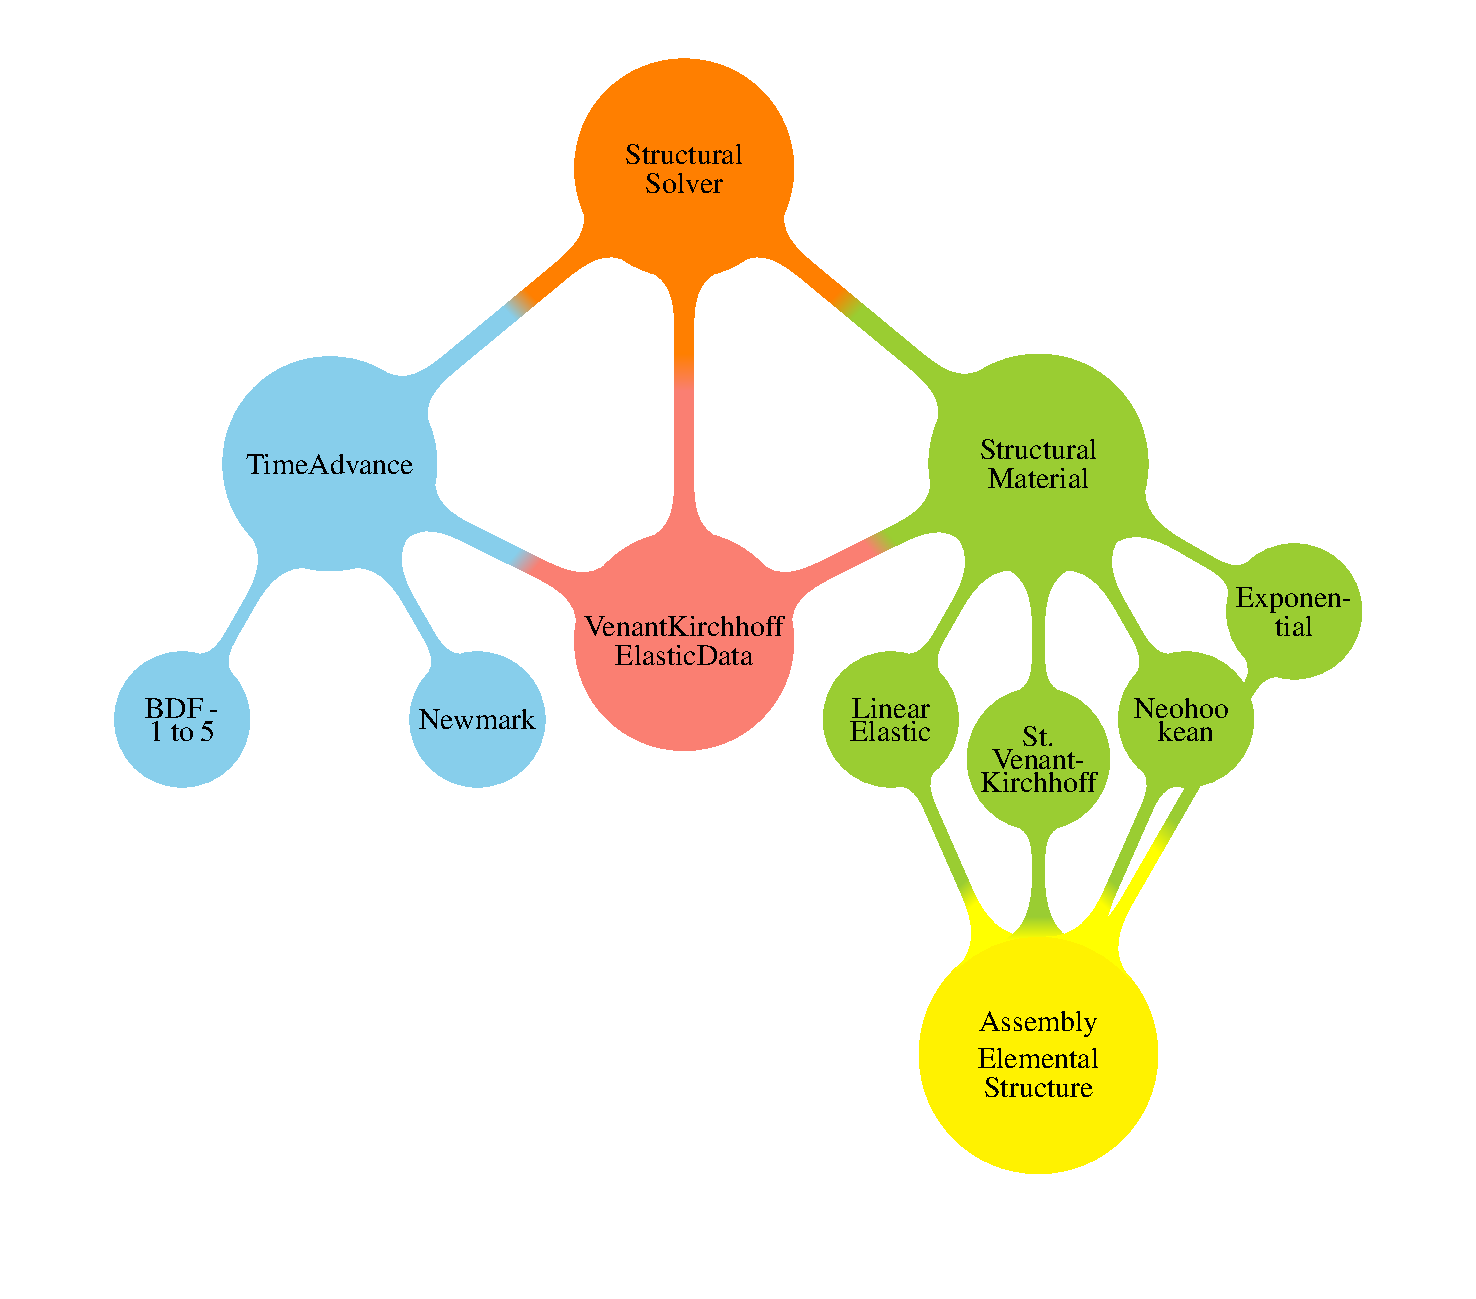
\includegraphics[width=14cm,height=12cm]{images/DesignStructural.pdf}
  \caption{Schematic representation of the main characters of the
    \SSol{} framework and of their interactions}
  \label{fig::design}
\end{figure}
\subsection{The \textit{StructuralSolver} class}
This class is the
solver of the structural mechanics problem. It has been developed
according to the common design pattern used for other solvers in
\LV. According to this, its main three methods are:
\begin{itemize}
\item \tPC{buildSystem()},
\item \tPC{updateSystem()},
\item \tPC{iterate()}.
\end{itemize}
The first builds the mass matrix \mass (which is
constant for all the time steps). The second one updates the right hand
side of the system \eqref{eq::GeneralSystem} and the last solves the
nonlinear system:
\begin{equation}
  \LE\left(\vectL^{n+1}\right)=0
  \label{eq::Root}
\end{equation}
The \tPC{iterate} method contains the Newton method
applied to \eqref{eq::Root}. The three main steps of the Newton method
are:
\begin{itemize}
\item evaluating the residual using the displacement field at the
  iteration $k$ of the Newton method. This stage is implemented in
  \tPC{StructuralSolver::evalResidual()};
\item updating the Jacobian using the displacement field at the
  current iteration $k$. It is implemented in
  \tPC{StructuralSolver::updateJacobian()};
\item solving the linearized system. The method
  \tPC{StructuralSolver::solveJacobian()} implements this stage.
\end{itemize} In order to solve the mathematical problem
\eqref{eq::MathProb}, this solver communicates with three main
classes:
\begin{itemize}
\item \tPC{StructuralMaterial},
\item \tPC{VenantKirchhoffElasticData},
\item \tPC{TimeAdvance}.
\end{itemize}
The \tPC{StructuralMaterial} class defines the
constitutive law which is used during the simulation. The second class
contains the mechanical parameters of the material (e.g. Young
modulus, Poisson ratio) and some useful variables set in the data file
of the simulation. The last class, as anticipated in \ref{sct-Linear},
manages the time advancing procedure and it is not described here.\\

\subsection{The \textit{StructuralMaterial} class} This is the core of
the new framework. It has been designed to be a general interface
between all the material models and the solver class. In this way, the
different structural models can be used in a very flexible way just
changing a variable, called solidType, in the data file.\\ For this
reason, from the practical point of view, this class is a factory (see
\cite{DesignPattern}). It has only virtual methods and the most
important are:
\begin{itemize}
\item \tPC{computeStiffness()},
\item \tPC{updateJacobianMatrix()}.
\end{itemize}
Since they are pure virtual methods, in each class
corresponding to a structural model there is the specific
implementation of the two methods above according to the chosen law.\\
The method \tPC{computeStiffness()} computes, using the displacement
fields at the iteration $k$ of the Newton method, the stiffness vector
when the solver class has to evaluate the residual in
\tPC{evalResidual()}. The second method provides StructuralSolver
with the Jacobian matrix of \Piola.\\

\subsection{The \textit{AssemblyElementalStructure}
  \texttt{namespace}}
As it will be shown later on, lots of new methods
have been developed to compute all the terms of the first
Piola-Kirchhoff tensor and its Jacobian for all the material models.
\AES{} is a new namespace defined in \LV. Its creation was necessary in
order to keep all these new methods separated from the ones which had
been previously developed (for different purposes) and grouped in the
AssemblyElemental namespace. Few methods, which were already available
in \LV{} in AssemblyElemental have been kept and not doubled in the new
namespace. When those methods are used, the interested reader may
refer to their definition in the AssemblyElemental namespace in
\tPC{AssemblyElemental.hpp}.\\ As it can be seen from
Fig. \ref{fig::design}, \AES{} is used only by the classes of the
material laws, that is where \Piola{} and the Jacobian are computed.



\subsection{Implementation of the different constitutive relations} In
this section we give a detailed description of the implementation of
the structural models. All the methods in the following receive some
arguments from the class that calls them. Here we will neglect all of
them. The interested reader may refer directly to their implementation
to have more details on this.


\subsubsection{The St. Venant-Kirchhoff model} This model is
implemented in \tPC{VenantKirchhoffMaterialNonLinear.hpp}. We will
refer to Eq. \eqref{eq::SVK-P-displ} for the definitions of the
methods.\\ The correspondance between the terms in
Eq. \eqref{eq::SVK-P-displ} and their implementation is:
\begin{itemize}
\item $\displaystyle \lambda(\diver{\displL})\I$ corresponds to
  \tPC{stiff\_div},
\item $\displaystyle \mu\big(\delOp\displL + \delOp\displL^T\big)$
  corresponds to \tPC{stiff\_strain},
\item $\displaystyle
  \frac{\lambda}{2}\big(\delOp\displL:\delOp\displL\big)$ corresponds to
  \tPC{stiff\_derdiv},
\item $\displaystyle \lambda\big(\diver{\displL}\big)\delOp\displL$
  corresponds to \tPC{stiff\_divgrad},
\item $\displaystyle
  \frac{\lambda}{2}\big(\delOp\displL:\delOp\displL\big)\delOp\displL$
  corresponds to \tPC{stiff\_gradgrad},
\item $\displaystyle \mu\big(\delOp\displL^T \delOp\displL\big)$
  corresponds to \tPC{stiff\_dergradbis},
\item $\displaystyle
  \mu\delOp\displL\big(\delOp\displL\delOp\displL^T\big)$ is splitted
  into the sum of two members. The first one corresponds to
  \tPC{stiff\_dergrad\_gradbis.} The second is
  \tPC{stiff\_dergrad\_gradbis\_Tr},
\item $\displaystyle \mu\delOp\displL\delOp\displL^T\delOp\displL$
  corresponds to \tPC{stiff\_gradgradTr\_gradbis}.
\end{itemize}
The definition of the Jacobian on \Piola{} is given in
Eq. \eqref{eq::SVK-Jacobian}. Here we specify the implementations of
the terms:
\begin{itemize}
\item $\displaystyle \lambda(\delOp\cdot\delta\Spost)$ corresponds
  to \tPC{stiff\_div},
\item $\displaystyle \mu(\delOp\delta\Spost +
  (\delOp\delta\Spost)^T)$ corresponds to \tPC{stiff\_strain},
\item $\displaystyle \lambda\delOp\Spost:\delOp\delta\Spost$
  corresponds to \tPC{stiff\_derdiv},
\item $\displaystyle \lambda(\delOp\cdot\Spost)\delOp\delta\Spost$
  corresponds to \tPC{stiff\_divgrad},
\item $\displaystyle \lambda(\delOp\cdot\delta\Spost)\delOp\Spost$
  corresponds to \tPC{stiff\_divgrad\_2},
\item $\displaystyle
  \frac{\lambda}{2}(\delOp\delta\Spost:\delOp\Spost)\delOp\Spost$ and
  the term $\displaystyle
  \frac{\lambda}{2}(\delOp\Spost:\delOp\delta\Spost)\delOp\Spost$ are
  added up in \tPC{stiff\_gradgrad\_2},
\item $\displaystyle
  \frac{\lambda}{2}(\delOp\Spost:\delOp\Spost)\delOp\delta\Spost$
  corresponds to \tPC{stiff\_gradgrad},
\item $\displaystyle \mu(\delOp\Spost)^{\text{T}}\delOp\delta\Spost$
  and the term $\displaystyle
  \mu(\delOp\delta\Spost)^{\text{T}}\delOp\Spost$ are added up and
  implemented in \tPC{stiff\_dergrad},
\item $\displaystyle \mu\delOp\Spost\delOp\delta\Spost$ corresponds
  to \tPC{stiff\_dergrad\_gradbis},
\item $\displaystyle \mu\delOp\delta\Spost\delOp\Spost$ corresponds
  to \tPC{stiff\_dergrad\_gradbis\_2},
\item $\displaystyle \mu\delOp\Spost(\delOp\delta\Spost)^{\text{T}}$
  corresponds to \tPC{stiff\_dergrad\_gradbis\_Tr},
\item $\displaystyle \mu\delOp\delta\Spost(\delOp\Spost)^{\text{T}}$
  corresponds to \tPC{stiff\_dergrad\_gradbis\_Tr\_2},
\item $\displaystyle
  \mu\delOp\delta\Spost(\delOp\Spost)^{\text{T}}\delOp\Spost$
  corresponds to \tPC{stiff\_gradgradTr\_gradbis\_3},
\item $\displaystyle
  \mu\delOp\Spost(\delOp\delta\Spost)^{\text{T}}\delOp\Spost$
  corresponds to \tPC{stiff\_gradgradTr\_gradbis\_2},
\item $\displaystyle
  \mu\delOp\Spost(\delOp\Spost)^{\text{T}}\delOp\delta\Spost$
  corresponds to \tPC{stiff\_gradgradTr\_gradbis}.
\end{itemize}


\subsubsection{The Linear Elastic model} This constitutive law is
defined in \tPC{VenantKirchhoffMaterialLinear.hpp}. We recall the
definition of \Piola{} as a function of the displacement field,
Eq. \eqref{eq::LE-P}.\\ Herein there is the list of the
correspondances:
\begin{itemize}
\item $\lambda(\diver{\displL})\I$ corresponds to the method
  \tPC{stiff\_div};
\item $\mu\big(\delOp\displL + \delOp\displL^T\big)$ corresponds to
  the method \tPC{stiff\_strain}.
\end{itemize}
In the case of linear elastic model, the Jacobian of
\Piola{} is the tensor itself and for this reason it is not
specified. The methods listed above belong to the AssemblyElemental
namespace since this constitutive law was already available in \LV{}
before the creation of the \SSolNC{} framework.


\subsubsection{The Neohookean model} The first Piola-Kirchhoff tensor
is defined in Eq. \eqref{eq::NH-P}. The terms have been implemented in
different methods as follows:
\begin{itemize}
\item $\displaystyle \mu
  J^{-\frac{2}{3}}\left(\F-\frac{1}{3}I_{\C}\F^{-T}\right)$ in the
  method \tPC{source\_P1iso\_NH},
\item $\displaystyle
  J\frac{\kappa}{2}\left(J-1+\frac{1}{J}\text{ln}J\right)\F^{-T}$ in the
  method \tPC{source\_Pvol}.
\end{itemize}
Concerning the Jacobian, defined in
Eqs. \eqref{eq::IsoPartDP-neo} and \eqref{eq::VolPartDP-neo}, the
implementation for the isochoric part has been done has follows:
\begin{itemize}
\item $\displaystyle
  -\frac{2}{3}J^{-\frac{5}{3}}\left(\cofF:\GradSpost\right)\F$ in
  \tPC{stiff\_Jac\_P1iso\_NH\_1term},
\item $\displaystyle \frac{2}{9}\mu
  J^{-2}I_{\C}\left(\cofF:\GradSpost\right)\cofF$ in
  \tPC{stiff\_Jac\_P1iso\_NH\_2term},
\item $\displaystyle \frac{2}{3}\mu
  J^{-\frac{5}{3}}\left(\F:\GradSpost\right)\cofF$ in
  \tPC{stiff\_Jac\_P1iso\_NH\_3term},
\item $\displaystyle \mu J^{-\frac{2}{3}}\GradSpost$ in
  \tPC{stiff\_Jac\_P1iso\_NH\_4term},
\item $\displaystyle
  \frac{\mu}{3}J^{-2}I_{\C}\cofF\GradSpost^T\cofF$ in
  \tPC{stiff\_Jac\_P1iso\_NH\_5term}.
\end{itemize}
For the volumetric part, these methods have been
created:
\begin{itemize}
\item $\displaystyle
  \frac{\kappa}{2}\left(2J^2-J+1\right)\left[\F^{-T}:\GradSpost\right]\F^{-T}$
  in \tPC{stiff\_Jac\_Pvol\_1term},
\item $\displaystyle
  \frac{\kappa}{2}\left(J-J^2-\text{ln}(J)\right)\F^{-T}\GradSpost^T\F^{-T}$
  in \tPC{stiff\_Jac\_Pvol\_2term}.
\end{itemize}


\subsubsection{The Exponential model} In this case we analyze only the
isochoric part of \Piola{} (Eq. \eqref{eq::EXP-P}). It is composed only
by one term,
\begin{displaymath}
  \displaystyle \alpha
  J^{-\frac{2}{3}}\left(\F-\frac{1}{3}I_{\C}\F^{-T}\right)
  e^{\gamma\big(I_{\C}-3\big)},
\end{displaymath}
and it has been implemented in the method
\tPC{source\_P1iso\_Exp}.  The correspondance between the terms of the
isochoric part of the Jacobian (Eq. \eqref{eq::IsoPartDP-exp}) and
their own implementations in AssemblyElementalStructure is:
\begin{itemize}
\item $\displaystyle -\frac{2}{3}\alpha\term
  J^{-\frac{5}{3}}\left(1+\gamma
    I_{\C}\right)\left[\cofF:\GradSpost\right]\F$ corresponds to
  \tPC{stiff\_Jac\_P1iso\_Exp\_1term},
\item $\displaystyle 2\alpha\gamma\term J
  ^{-\frac{4}{3}}\left(\F:\GradSpost\right)\F$ corresponds to
  \tPC{stiff\_Jac\_P1iso\_Exp\_2term},
\item $\displaystyle \frac{2}{9}\alpha\term
  J^{-2}I_{\C}\left(1+\gamma
    I_{\C}\right)\left(\cofF:\GradSpost\right)\cofF$ corresponds to
  \tPC{stiff\_Jac\_P1iso\_Exp\_3term},
\item $\displaystyle -\frac{2}{3}\alpha\term
  J^{-\frac{5}{3}}\left(1+\gamma
    I_{\C}\right)\left(\F:\GradSpost\right)\cofF$ corresponds to
  \tPC{stiff\_Jac\_P1iso\_Exp\_4term},
\item $\displaystyle \alpha\term J^{-\frac{2}{3}}\GradSpost$
  corresponds to \tPC{stiff\_Jac\_P1iso\_Exp\_5term},
\item $\displaystyle \frac{\alpha}{3}\term
  J^{-2}I_{\C}\cofF\GradSpost^T\cofF$ corresponds to
  \tPC{stiff\_Jac\_P1iso\_Exp\_6term}.
\end{itemize}
The volumetric part in both the first Piola-Kirchhoff
tensor and in its Jacobian, is the same for the Neohookean and
Exponential model. For this reason, it has not been specified here.

\section{The \tSS and validation}
This section describes the \tSS that has been inserted in the testsuite folder of the library. It shows the numerical validation that has been carried out in order to assure that the numerical solver works properly.

The \tSS implements the steady case of homogeneous pure strain of a cube. The problem reads as follows:
\begin{equation}
\left\{
\begin{array}{lllllll}
  \displaystyle \text{Div}(\Piola) + \rho_0\underline{b} = \underline{0} & \text{on} \quad [0,L]^3,\\
  \\
  \displL(t)=\underline{0} & \text{on} \quad \Gamma_D, \quad t>0,\\
  \Piola\underline{n}_2=\underline{t}_0 & \text{on} \quad \Gamma_{N_2}, \quad t>0.\\
\end{array}\right.
\label{eq::homStrain}
\end{equation}
where $L$ is the length of the cube side. Fig.~\ref{fig::pureStrain} is the two dimensional representation of \eqref{eq::homStrain}. As represented in the figure, the applied stress has only nonzero component along the axis perpendicular to the surface. 
\begin{figure}
  \centering
  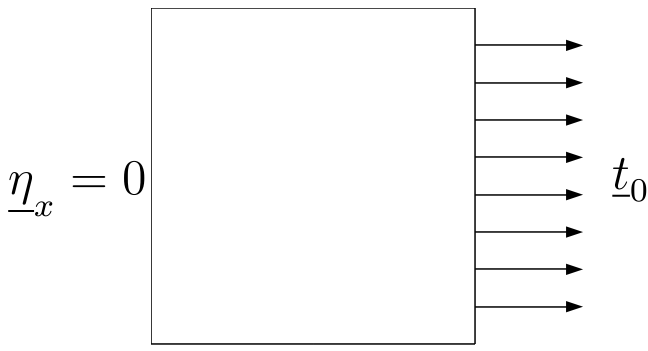
\includegraphics[width=0.35\textwidth]{images/modelProblem.png}
  \caption{2D representation of Problem \eqref{eq::homStrain}}
  \label{fig::pureStrain}
\end{figure}
\begin{figure}
  \centering
  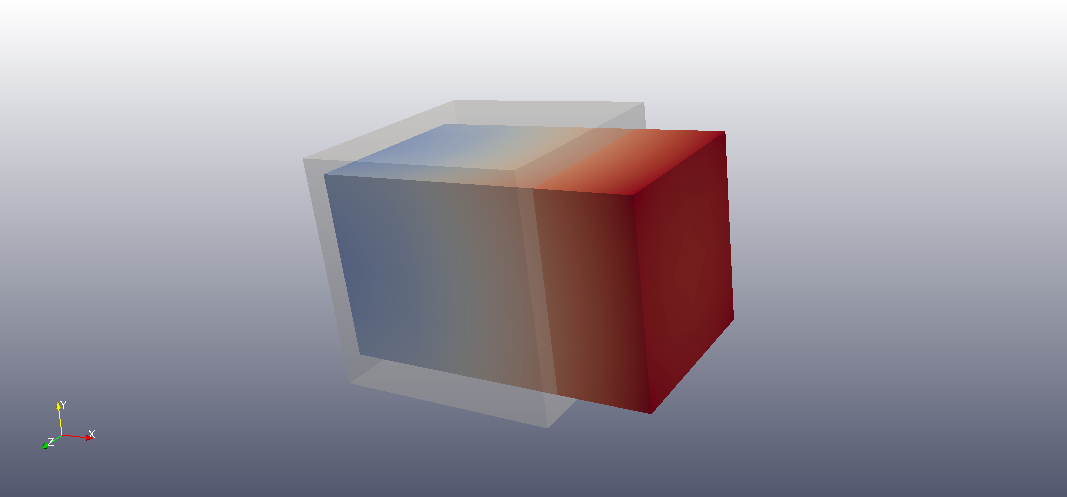
\includegraphics[width=0.45\textwidth]{images/cube_exp_timeAdvance-BDF1.png}
  \caption{Deformation of the cube under the applied traction}
  \label{fig:displ}
\end{figure}

Fig.\ref{fig:displ} shows the deformation of the cube under the applied traction. The simple model problem \eqref{eq::homStrain} allows to find an analytical expression of the first Piola-Kirchhoff tensor. In this case, the deformation gradient \F and the right Cauchy-Green tensor \C read
\begin{equation}
  \F = \left(
  \begin{array}{ccc}
    \lambda_1 & 0 & 0 \\
    0 & \lambda_2 & 0 \\
    0 &  0  & \lambda_3 
  \end{array}\right)\qquad\quad
  \C = \left(
  \begin{array}{ccc}
    \lambda_1^2 & 0 & 0 \\
    0 & \lambda_2^2 & 0 \\
    0 &  0  & \lambda_3^2 
  \end{array}\right)
\end{equation}
In this case, the invariants of \C depend only on the deformations $\lambda_i$. Consequently, according to \eqref{eq::WandInvariants} the function \W depends on the diagonal elements of \F. Moreover, \W satisfy the simmetries
\begin{equation}
  \WE(\lambda_1,\lambda_2,\lambda_3)=\WE(\lambda_1,\lambda_2,\lambda_3)=\WE(\lambda_1,\lambda_3,\lambda_2)=\WE(\lambda_3,\lambda_1,\lambda_2).
  \label{eq::W&Lambda}
\end{equation}
Furthermore, due to the simmetry of the test case, $\lambda_2=\lambda_3$ and they can be derived by the determinant of \F thanks to the relation
\begin{equation}
  \displaystyle \lambda_2=\lambda_3=\sqrt{\frac{J}{\lambda_1}},
  \label{eq::diffLambda}
\end{equation}
where $J=\text{det}\F$. Inserting \eqref{eq::diffLambda} in \eqref{eq::W&Lambda}, the general form of \W becomes
\begin{equation}
\displaystyle \WE=\WE(\lambda_1,\sqrt{\frac{J}{\lambda_1}}\big).
\label{eq::syntW}
 \end{equation}
Thanks to \eqref{eq::syntW}, it is possible to compute the first Piola-Kirchhoff tensor analitically. In particular, the exact expression of the  term $\Piola_{11}$ can be deduced. Since the determinant $J$ is present in \eqref{eq::syntW}, we consider also the term $\Piola_{22}$. In the following, the expression of $\Piola_{11}$ for the three constitutive laws is provided:
\begin{itemize}
  \item \textit{St. Venant-Kirchhoff}:
    \begin{equation}
      \begin{array}{lll}
      & \Piola_{11}=\displaystyle \frac{\lambda}{2}(I_{\C}-3)\lambda_1 - \mu\lambda_1 + \mu\lambda_1^3;\\
      \\
      & \Piola_{22}=\displaystyle \frac{\lambda}{2}(I_{\C}-3)\lambda_2 - \mu\lambda_2 + \mu\lambda_2^3;
      \end{array}
      \label{eq::P11SVK}
    \end{equation}
  \item \textit{Neo-Hookean}:
    \begin{equation}      
      \begin{array}{lll}
      & \Piola_{11}=\displaystyle \mu J^{-2/3} (\lambda_1 - \frac{I_{\C}}{3\lambda_1}) + \frac{\kappa}{2}(J^2 - J + log(J))\frac{1}{\lambda_1};\\
      \\
      & \Piola_{22}=\displaystyle \mu J^{-2/3} (\lambda_1 - \frac{I_{\C}}{3\lambda_2}) + \frac{\kappa}{2}(J^2 - J + log(J))\frac{1}{\lambda_2};
      \end{array}
      \label{eq::P11NH}
    \end{equation}
  \item \textit{Exponential}:
    \begin{equation}
      \begin{array}{lll}
      & \Piola_{11}=\displaystyle \alpha \term J^{-2/3}(\lambda_1 - \frac{I_{\C}}{3\lambda_1})+\frac{\kappa}{2}(J^2 - J + log(J))\frac{1}{\lambda_1};\\
      \\
      & \Piola_{22}=\displaystyle \alpha \term J^{-2/3}(\lambda_2 - \frac{I_{\C}}{3\lambda_2})+\frac{\kappa}{2}(J^2 - J + log(J))\frac{1}{\lambda_2};
      \end{array}
      \label{eq::P11EXP}
    \end{equation}
\end{itemize}
The procedure that has been followed is the following:
\begin{enumerate}
  \item a specific traction is applied on the Neumann face of the cube and the deformation $\lambda_1$ is obtained numerically; 
  \item the term $\Piola_{22}$ is equal to zero and then, the expression of $J$ as a function of $\lambda_1$ can be computed.
  \item the function $J=J(\lambda_1)$ is introduced in one of the three expressions of $\Piola_{11}$ according to the choosen constitutive law and the value of $\Piola_{11}$ deduced. If the code works properly, the value of $\Piola_{11}$ using the computed deformation is equal to the applied traction.
\end{enumerate}
The numerical test has been carried out on a structured mesh of 125 nodes. The polynomial space is P1. The material parameters are the following:
\begin{itemize}
  \item \textit{Poisson ratio} $= 0.45$;
  \item \textit{Young modulus} $= 6e6$;
  \item $\kappa$ $=1e8$; 
  \item $\alpha$ $=2e6$; 
  \item $\gamma$ $=0.80$; 
\end{itemize}
After having obtained the deformation $\lambda_1$ and computed the corresponding term in \Piola, the relative error
\begin{equation}
  err = \displaystyle \frac{\Piola_{11-analitical}-\Piola_{11-numerical}}{\Piola_{11-analitical}},
\end{equation}
where $\Piola_{11-analitical}$ is the applied traction force and $\Piola_{11-numerical}$ is the stress computed using the procedure explained above, has been analyzed.

Figs.\ref{fig:errLE},\ref{fig:errSVK},\ref{fig:errNH},\ref{fig:errEXP} show the comparisons between the analytical and numerical relation between $\Piola_{11}$ and the behaviour of the relative error when different loads are applied and, consequently, different deformations are obatined.

\begin{figure}[h!]
\centering
\subfigure[Stress-Strain relation]{
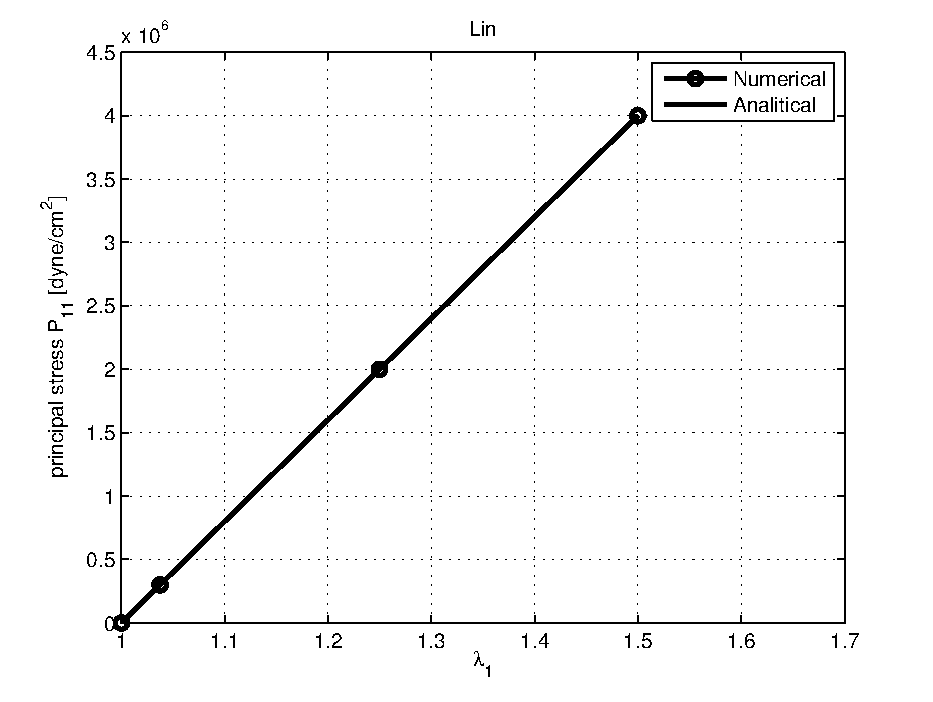
\includegraphics[width=0.32\textwidth]{images/sigepsP1-Lin-BDF1.pdf}}
\subfigure[Relative error]{
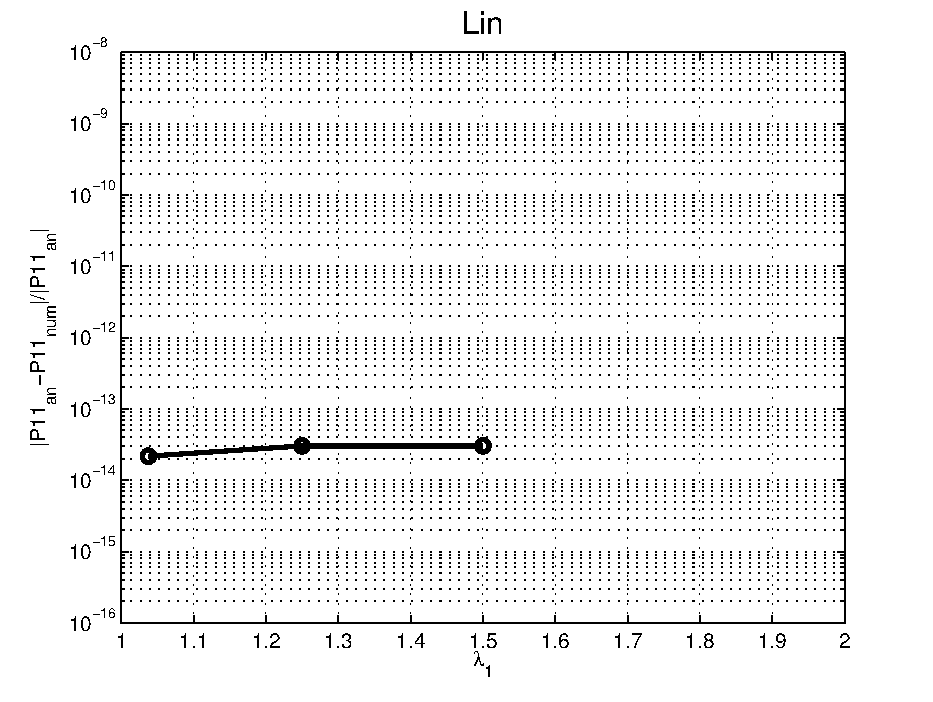
\includegraphics[width=0.32\textwidth]{images/errorP1-Lin-BDF1.pdf}}
\caption{Comparison between analytical and numerical solution for Linear Elastic}
\label{fig:errLE}
\end{figure}

\begin{figure}[h!]
\centering
\subfigure[Stress-Strain relation]{
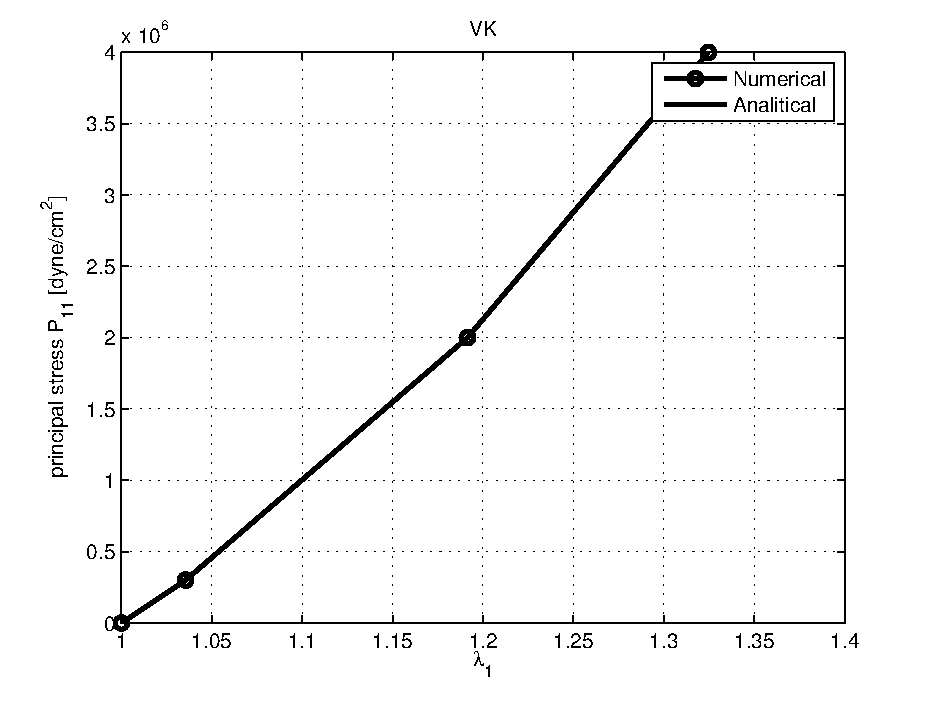
\includegraphics[width=0.32\textwidth]{images/sigepsP1-SVK-BDF1.pdf}}
\subfigure[Relative error]{
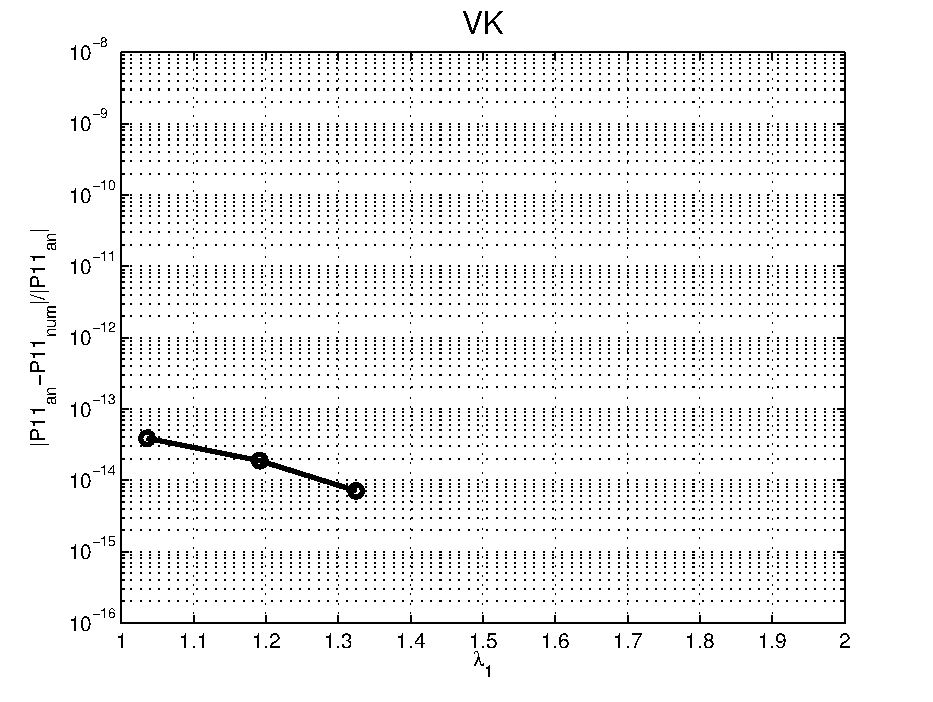
\includegraphics[width=0.32\textwidth]{images/errorP1-SVK-BDF1.pdf}}
\caption{Comparison between analytical and numerical solution for St. Venant-Kirchhoff}
\label{fig:errSVK}
\end{figure}

\begin{figure}[h!]
\centering
\subfigure[Stress-Strain relation]{
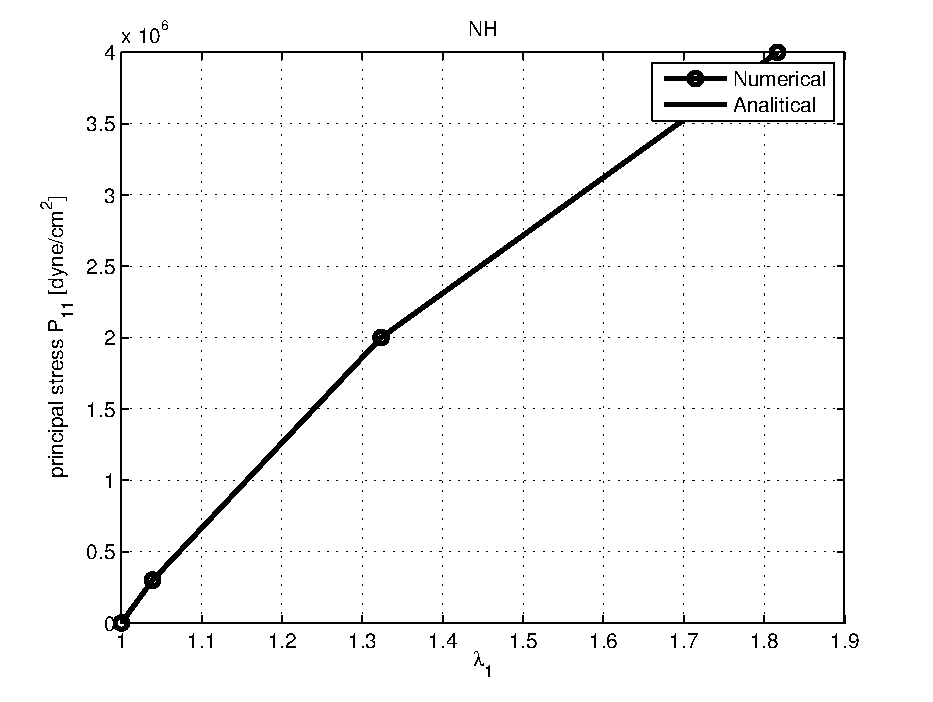
\includegraphics[width=0.32\textwidth]{images/sigepsP1-NH-BDF1.pdf}}
\subfigure[Relative error]{
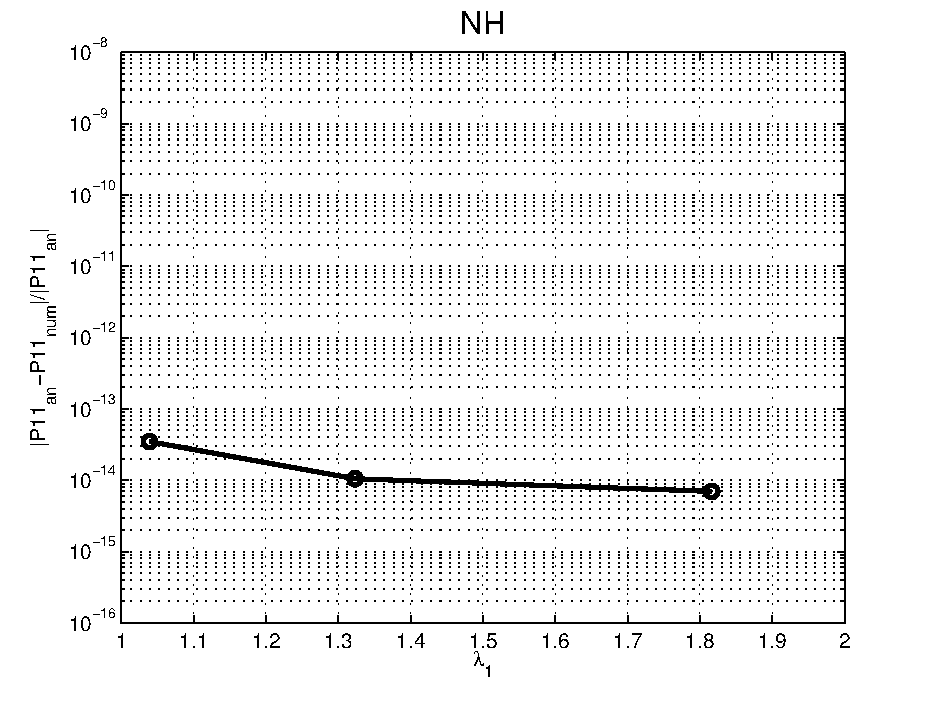
\includegraphics[width=0.32\textwidth]{images/errorP1-NH-BDF1.pdf}}
\caption{Comparison between analytical and numerical solution for Neo-Hookean}
\label{fig:errNH}
\end{figure}

\begin{figure}[h!]
\centering
\subfigure[Stress-Strain relation]{
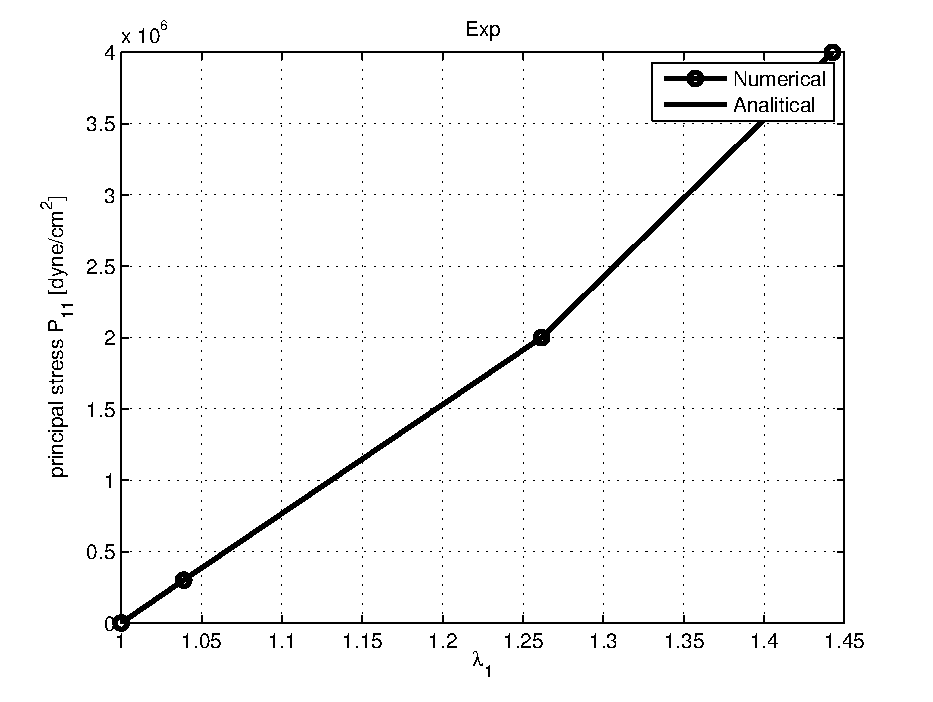
\includegraphics[width=0.32\textwidth]{images/sigepsP1-EXP-BDF1.pdf}}
\subfigure[Relative error]{
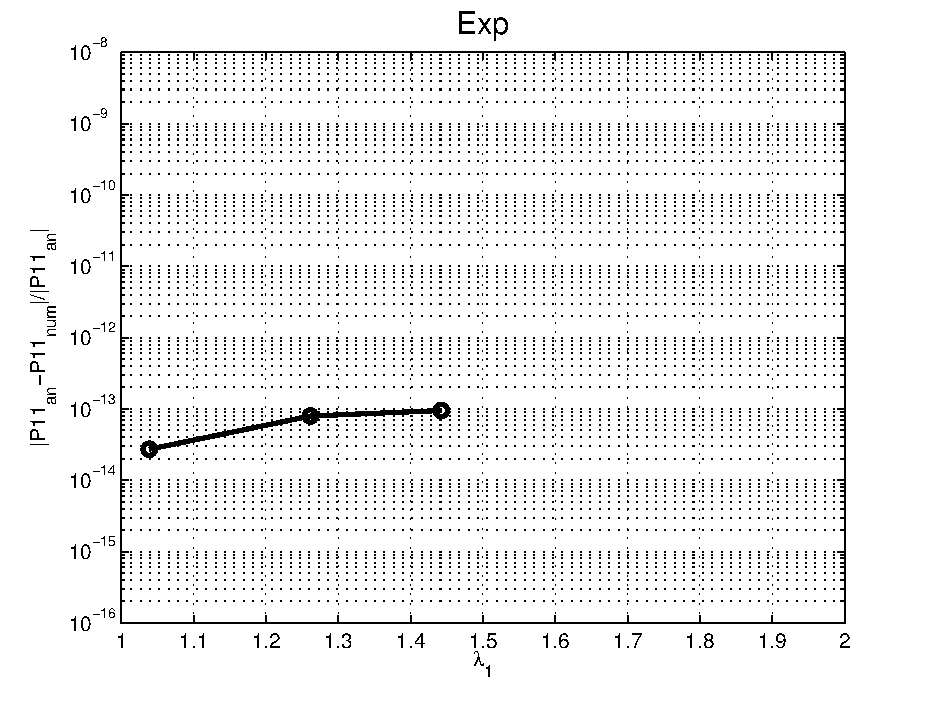
\includegraphics[width=0.32\textwidth]{images/errorP1-EXP-BDF1.pdf}}
\caption{Comparison between analytical and numerical solution for exponential}
\label{fig:errEXP}
\end{figure}



\bibliographystyle{plain}
\bibliography{StructuralSolver}
\addcontentsline{toc}{section}{Bibliography}

\end{document}
